\documentclass[10pt,twocolumn,letterpaper]{article}

\usepackage{cvpr}
\usepackage{times}
\usepackage{epsfig}
\usepackage{graphicx}
\usepackage{amsmath}
\usepackage{amssymb}
\usepackage{xcolor}
\usepackage{tabularx}
\usepackage{array}
\newcolumntype{M}[1]{>{\centering\arraybackslash}m{#1}}
\newcolumntype{L}[1]{>{\raggedleft\arraybackslash}m{#1}}

% Include other packages here, before hyperref.

% If you comment hyperref and then uncomment it, you should delete
% egpaper.aux before re-running latex.  (Or just hit 'q' on the first latex
% run, let it finish, and you should be clear).
\usepackage[breaklinks=true,bookmarks=false]{hyperref}

\cvprfinalcopy % *** Uncomment this line for the final submission

\def\cvprPaperID{****} % *** Enter the CVPR Paper ID here
\def\httilde{\mbox{\tt\raisebox{-.5ex}{\symbol{126}}}}

% Pages are numbered in submission mode, and unnumbered in camera-ready
%\ifcvprfinal\pagestyle{empty}\fi
\setcounter{page}{1}
\begin{document}

%%%%%%%%% TITLE
\title{Facial expression recognition application using CNNs}

\author{
Peagno Eleonora \\\normalsize 1237035\\
%{\tt\small }
% For a paper whose authors are all at the same institution,
% omit the following lines up until the closing ``}''.
% Additional authors and addresses can be added with ``\and'',
% just like the second author.
% To save space, use either the email address or home page, not both
\and
Peron Giovanni \\\normalsize 1237783\\
%{\tt\small secondauthor@i2.org}
\and
Rossi Daniel \\\normalsize 1211017\\
%{\tt\small secondauthor@i2.org}
}

\maketitle
%\thispagestyle{empty}

%%%%%%%%% ABSTRACT
\begin{abstract}
   %The ABSTRACT is to be in fully-justified italicized text, at the top
   %of the left-hand column, below the author and affiliation
   %information. Use the word ``Abstract'' as the title, in 12-point
   %Times, boldface type, centered relative to the column, initially
   %capitalized. The abstract is to be in 10-point, single-spaced type.
   %Leave two blank lines after the Abstract, then begin the main text.
   %Abstract should be no longer than 300 words.
   The facial expression recognition is a challenging task in machine learning field, 
   and there is an active research on this topic. Being able to make a machine understand 
   the human emotions is a fascinating goal.
   The purpose of this report is to exploit all the topics studied during 
   the Vision and Cognitive Services course and others like Machine Learning and Deep Learning
   in order to implement a system able to predict human emotions.
   We will describe how we realized this system specifying all the steps performed,
   from the first CNN we tried to the final model we obtained. 
   We will illustrate all the procedure we used trying to achieve better results.
   Our target was not very high since this is a challenging task as we said, however
   with our final model we arrived to a predition accuracy of \textbf{\textcolor{red}{...}} that is better than the human accuracy.
   Finally using this model we reached our goals implementing a nice application.
\end{abstract}

%%%%%%%%% BODY TEXT
\section{Introduction}
   Facial expressions recognition (FER) is an interesting and a challenging problem 
   in machine learning field. It is also a task that can be applied in many important applications.
   Facial expressions have an important role in every human interaction so having a machine able to 
   recognize and understand human expressions automatically can be very useful
   in many existing and novel fields \cite{2}.
   \\One of these fields is behaviomedics that are systems which exploit automatic analysis of affective and social signals 
   to aid diagnosis, monitoring and treating medical condition that alter behavior.
   Facial expression recognition can be also use in data analytics field for example to understand 
   emotions of people that are looking at ads or political debate and make statistics related to people's preferences. 
   Another application field for Facial expression recognition is human-computer interaction, understanding human emotions 
   would make the attitude of systems like vocal assistants or robots much closer to the way that humans interact with each other.
   Recognizing expressions could also be useful to improve the identification of micro facial expressions which can be used in 
   deceit detection applications.
   Due to all these possible applications, facial expressions recognition is widely studied also because recognizing 
   human expressions in natural condition environment is a very challenging task.
   With this project we aim to build a facial expressions classifier able to reach and overtake the human accuracy on this task. 
   The main idea was focusing mostly on study different types of model in order to understand a good way to achieve valid outcomes.
   For this reason all preprocessing techniques that can be applied to the input data for improving classification results were not be consider.
   \begin{center}
      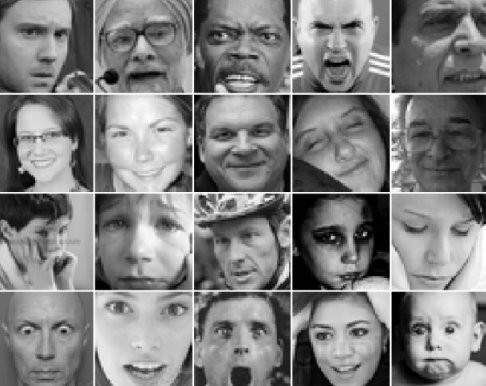
\includegraphics[width=0.8\linewidth]{./immagini/dataset.jpeg}
   \end{center}
   The chosen dataset is the FER2013 it was selected after some researches, above some examples of images of this dataset are reported. 
   FER2013 was the desired dataset, the most suited for our purpose. Training a model with a dataset like that was the challenge 
   with the right level of difficulty we wanted. 
   Moreover FER2013 provides a very large set of examples well differentiated in terms of person age, face pose, illumination and other realistic conditions.
   So using this dataset we realize an ensemble model using many types of Convolutional Neural Networks (CNNs), in order to achieve a test accuracy 
   greater than 65.5\%, that is the human accuracy measured on FER 2013 dataset \cite{3}. Our target was reached using the final model described in the next 
   sections, which achieve test accuracy of 71.52\% on FER2013. 

\section{Related Work}
The first step for reaching our targets it has been a research of all the scientific papers related to the facial expression recognition.
We found many different works related to the topic all reviewed in \textit{``Deep Facial Expression Recognition: A Survey''} by S. Li and W. Deng \cite{paper}, thank to this paper 
we could find a lot of different works about the same kind of classification we were looking for.
We searched for all the works reported that were using the FER2013 dataset, in order to understand a way to realize a model aligned with the best results achieved in the last years.
We found six different papers related to the FER2013 dataset, they were classified by accuracy reached and type of neural networks used. 
After inspecting all these works we chose to follow the paper that achieved the best accuracy, moreover it used an ensemble method and we were interested in understanding better this approach.
So we decided to follow the methods used in \textit{``Facial Expression Recognition using
Convolutional Neural Networks: State of the Art''} by C. Pramerdorfer and M. Kampel \cite{147}, that consists on an ensemble method made up eight different CNNs of three different types, the accuracy reported for this method was 75.2\%.
This paper has been enticing for us because in it are explained the power and the bottlenecks of the CNNs 
method, moreover the final part of that paper was destined to explain how is possible to overcome the problems of CNN.
We found also other papers that we used as support to realize many different types of Convolution Neural Networks:
\begin{itemize}
   \item ``Very Deep Convolutional Networks
   for Large-Scale Image Recognition'' by K. Simonyan and A. Zisserman \cite{24};
   \item ``Going Deeper with Convolutions'' by C. Szegedy, W. Liu, Y. Jia, P. Sermanet, S. Reed, D. Anguelov, D. Erhan,
   V. Vanhoucke, and A. Rabinovich \cite{13};
   \item ``Deep Residual Learning for Image Recognition'' by K. He, X. Zhang, S. Ren, and J. Sun \cite{5}.
\end{itemize}
Following we report a table that summarizes three of the works executing facial expressions 
recognition task on the FER2013 dataset, we considered from \cite{paper}. 

\begin{table}[h]
   \begin{center}
   \begin{tabular}{|M{2.2cm}|M{2.2cm}|M{1.6cm}|}
   \hline
   Papers & Network type & Accuracy reached\\
   \hline\hline
   Zhang et al. \cite{Zhang}& CNN Multitask Network& Test: 75.10\\\hline
   Kim et al. \cite{Kim}& CNN Network Ensemble & Test: 73.73\\\hline
   Pramerdorfer et al. \cite{147}& CNN Network Ensemble & Test: 75.2\\
   \hline
   \end{tabular}
   \end{center}
   \label{mytable}
\end{table}

\section{Dataset}
The FER2013 database was created by Pierre Luc Carrier and Aaron Courville. 
It was introduced during the ICML 2013 Challenges in Representation Learning, 
it is a large-scale and unconstrained database.
This dataset was builted collecting images in an automatic way using the Google image search API.
In order to find useful faces images 
a research has been carried out combining a set of emotion related keywords with other words associated
to gender, age or ethnicity. 
In this way about 600 strings were obtained and they were used to query the search API.
Then all the images collected with this system have been cropped and resized to 48*48 pixels
and they have been also converted to grayscale.
We choose this dataset for many reasons, for example we find it is cited in many papers and we consider it well formed dataset for the reason that it contains 
images which have different illumination, subjects with different age, pose and expression intensity, moreover some images
have also occlusions. In general the images contained in the FER2013 dataset represent a good sampling under realistic conditions. 
The most important reason that pushed us to choose it is the huge number of images that it provides.
Precisely it contains 28709 training images, 3589 validation images and 3589, so in total 35887 
images for each of them there is an associated class that represent seven different expression labels: Angry, Disgust, Fear, Happy, Sad, Surprised, Neutral.
Below we report an histogram showing the distribution of all the FER2013's labels.
\begin{center}
   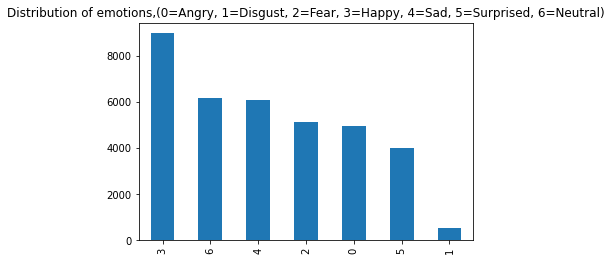
\includegraphics[width=1\linewidth]{./immagini/7_classi.png}
\end{center}
We tried to apply as few preprocessing techniques as possible because we want to focus on the model performance providing to it a dataset not too optimized.
We do this choice in order to emphasize the power of the model built, in the sense we want a model able to reach interesting performance independently
the goodness of the dataset provided to it.
For this reasons we operate only some minimal preprocessing modification over the dataset, in order to prepare the data to be learned. 
First of all we notice that the class disgust is not so big with respect to the others, so we decide to merge it with the angry class.
Following a graph showing the merged classes result.
\begin{center}
   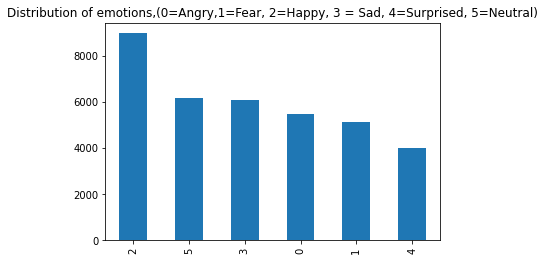
\includegraphics[width=1\linewidth]{./immagini/6_classi.png}
\end{center}
After this operation the classes are not so much leveled, in particular compared to happy class. 
In fact we have a lot of images for the happy class instead the ones for the surprised emotion are very few. 
To solve this issue we decide to replicate the 60\% of the images of each class, excluding the happy class because as we said it already has enough images.
In this way we make the images amount for each class more balanced and we reach the following distribution with a total amount of 52025 images. 
\begin{center}
   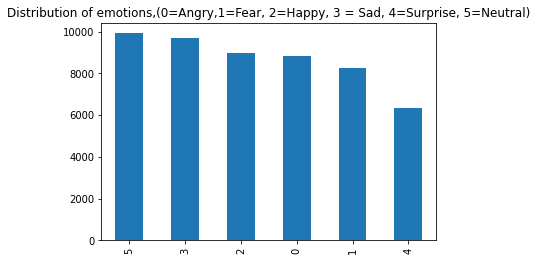
\includegraphics[width=1\linewidth]{./immagini/classi_bilanciate.png}
\end{center}
Finally we performed a normalization operation over the dataset in order to provide to the model a numeric common scale.
After all these needed preprocessing steps we obtain a training set formed by 44847 images and a test set and a validation set each one formed by 3589 images. 
\\An evaluation of other dataset has been done, we considered also CK+ (CohnKanade) dataset that is also commonly used for evaluating FER systems.
The first point that brought us to discard CK+ were the huge amount of data provided by FER2013 we decided to have more images as possible in order to 
obtain a model that could well generalize, moreover the aim of reaching an interesting accuracy with FER2013 was more challenging.
We decided to prefer FER2013 also because it appeared to us more easier to work with, in that FER2013 was provided in a csv file.
A more important reason that led us to prefer FER2013 is the fact this last provides specified training, validation and test sets, CK+ instead does not, so in order 
to compare our results with other works it was the most appropriate one.
\section{Method}
\section{Experiments}
\section{Conclusion}

We overtakes the accuracy reached from three papers which describe models that perform the same task with the same dataset used by us cited in \cite{paper}





{\small
\bibliographystyle{ieee_fullname}
\bibliography{egbib}
}

\end{document}
